\section{Example of use of XRM: The NURE Use Case}
\label{sec:conceptual-nure-example}

The conceptual model is a tool that could prove to be very powerful for the future development of XR applications: by providing a representation of the concepts that describe a certain phenomenon in an objective way, it is possible to let engineers, designers, researchers, technicians, museum curators etc. to be more focused on the requirements and goals of the project rather than trying to find a way to agree on the guidelines of the product to be developed. 

The XRM model also has this purpose: to enable multidisciplinary teams to collaborate in the most efficient way by introducing a set of primitives whose easy-to-understand nature makes communication between experts from different backgrounds immediate. In order to demonstrate its value, the XRM model has been applied in the design of an XR experience involving experts from different fields.
In this chapter, a case study is reported in order to provide an example related to the concepts introduced in the previous section. For this purpose, the MR experience of the archaeological site of NURE, designed in collaboration with the company FifthIngenium as a result of the ART project, was chosen. 
The next chapter (\autoref{subsec:art-editor-nure-example}) will show how a designer capable of interpreting the XRM model can easily reproduce the defined tasks and activities with the corresponding editor elements to obtain a complete specification of the experience flow in all its details.

The design process of NURE was iterative over a period of approximately 2 months and involved the FifthIngenium team composed by software engineers, graphic designers, expert archaeologists etc.

The XRM model was used as a common means of communicating and sharing ideas and proposals within the team. The design was organised in 3 steps: 
\begin{enumerate}
    \item Study and analysis of the document containing the site experts' on-site findings,
    \item Identification of the user profile as a visitor, of their needs and abilities and of the stakeholders' objectives 
    \item Identification of the involved elements of the experience and representation of them in terms of Non-Human Actors bearing in mind the chosen technologies. 
\end{enumerate}
Following this, we thought about the actions that the user can perform and the effects on the objects previously identified, laying the foundations for the definition of our Behavioural Model. Finally, after having defined all the primitives, it was not difficult to map the pre-defined building blocks to assemble the activities into which to divide the experience. 
As designers of NURE, we specified the Structural Model in which to insert all the identified protagonists, then the Behavioural Model listing all the User Actions and Effects needed and lastly the Interaction Model, in which we built and translated the Tasks and Activities into their graphical representation. In some cases we had to make assumptions as we could not interact directly with the technological devices that will be used. 
For obvious reasons of space, this section presents an example of the XRM-based modelling applied to the NURE experience. The site on which the NURE experience was built was divided into zones (\autoref{tab:orthophotoNURE}), and for each zone an Environment was planned (some contained sub-Environments) as shown in the \autoref{fig:ortophoto}.

\begin{figure}[h]
    \centering
    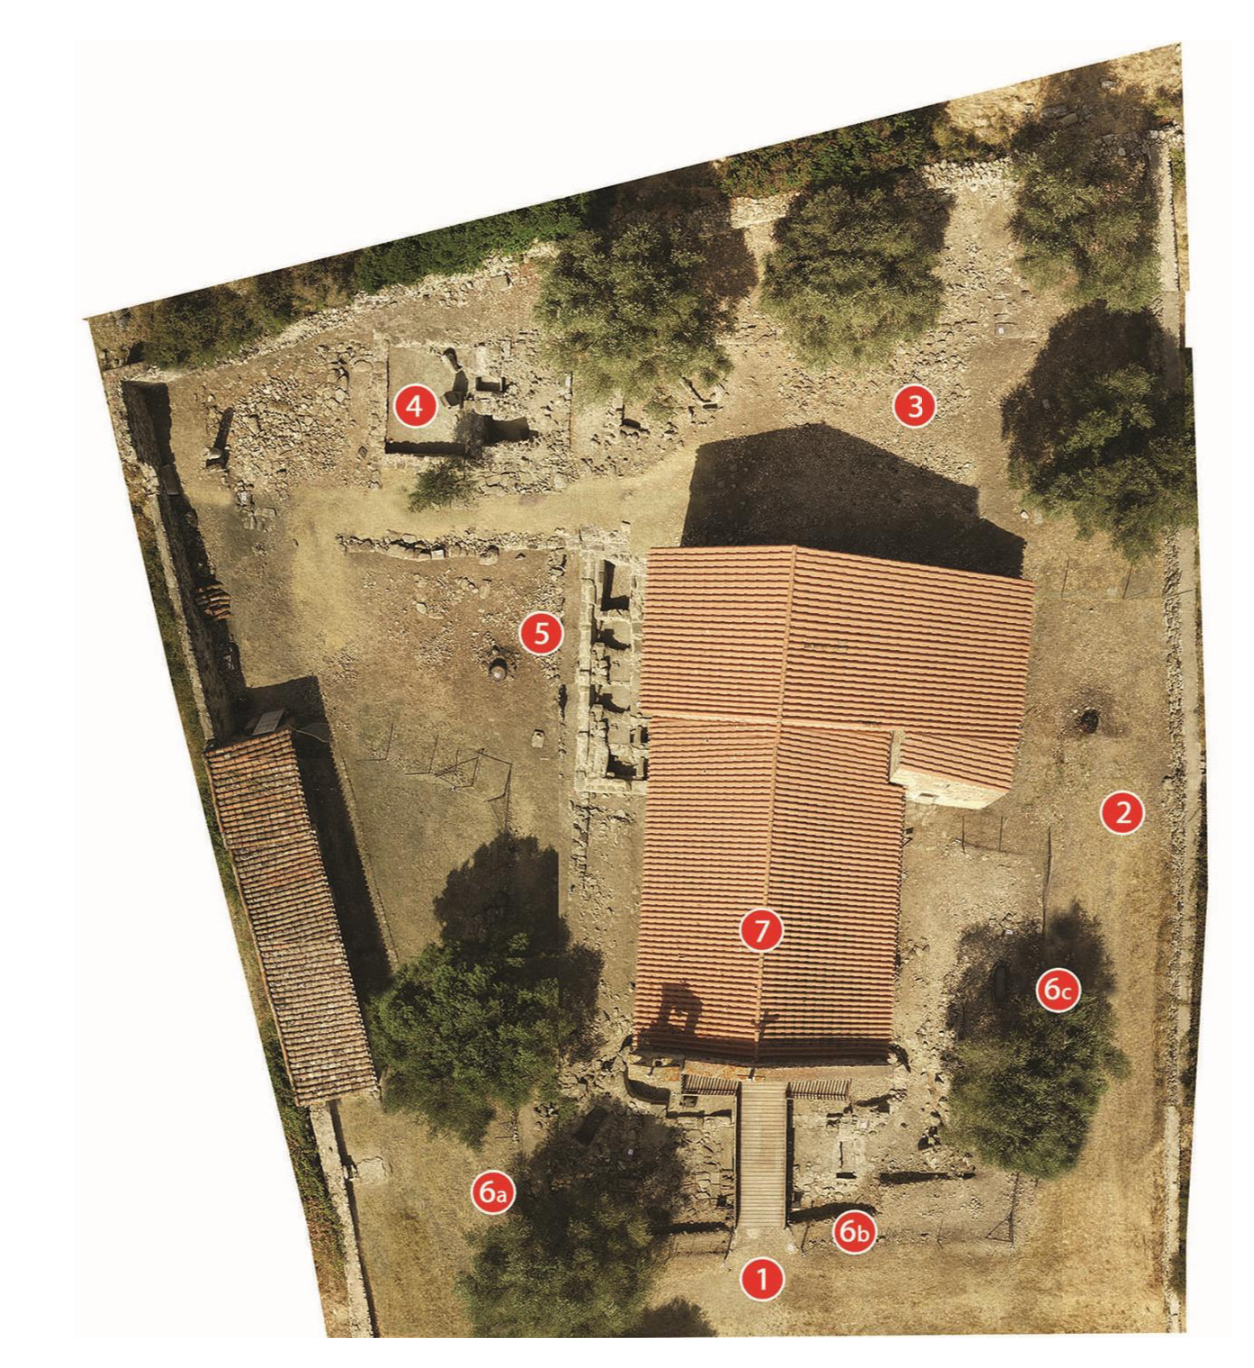
\includegraphics[width=\linewidth]{Figures/Conceptual Model/photoNURE/ortophoto.png}
    \caption{Site zones - NURE}
    \label{fig:ortophoto}
\end{figure}

\begin{table}[h]
\centering
\begin{tabular}{|l|l|}
\hline
\multicolumn{2}{|l|}{\textbf{Numbering and relocation of Environments on orthophotos}}                                                                        \\ \hline
1. & \begin{tabular}[c]{@{}l@{}}Paleochristian church, Mausoleum and Tombs \\ (D, E, H, L, R, T, Z) seen from the outside, from a distance.\end{tabular}      \\ \hline
2. & Nuraghe and 8 village huts seen from a distance.                                                                                                         \\ \hline
3. & Mausoleum (seen from outside) and pit Tombs D and E.                                                                                                     \\ \hline
4. & \begin{tabular}[c]{@{}l@{}}Mausoleum seen from the inside with a scene of the \\ Refrigerium rite performed by two women.\end{tabular}                   \\ \hline
5. &
  \begin{tabular}[c]{@{}l@{}}Chamber tomb H with hatch and barrel vault, and chamber\\ Tomb L with hatch and flat ceiling, located in the south wing \\ of the Early Christian church.\end{tabular} \\ \hline
6. & \begin{tabular}[c]{@{}l@{}}Masonry pit tomb R, masonry pit Tomb T and sarcophagus \\ Tomb Z, located near the east elevation of the church.\end{tabular} \\ \hline
7. &
  \begin{tabular}[c]{@{}l@{}}Interior of the early Christian church with a view of the nave, \\ side aisles, ciborium, presbytery, altar, apse, well and nuragic \\ hut under the main nave.\end{tabular} \\ \hline
\end{tabular}
\caption{Environments on Orthophotos - NURE}
\label{tab:orthophotoNURE}
\end{table}

\subsubsection*{Structural Model - NURE}

\emph{Actors}. The Human Actors of the NURE case study is the visitor who wants to enjoy a tour of the archaeological park (\autoref{fig:ActorsNURE}). The identified Non-Human Actors belong to the sub-hierarchies of Physical Components, Environment and Virtual Objects (\autoref{fig:NonHumanActorsNURE}). In this section we describe the Non-Human Actors at the lower level with the intention of giving a demonstration of how the Structural Model was applied. In addition, we report in the following tables some of the properties of the individual Actors. It is to be considered that the properties are intended in their initial state, since Actors, as Targets of the Interaction, undergo changes at a structural level that become evident only when they become Actuators, i.e. when the User Action has generated a certain effect on a Non-Human Actor.

\begin{figure}[H]
	\centering
	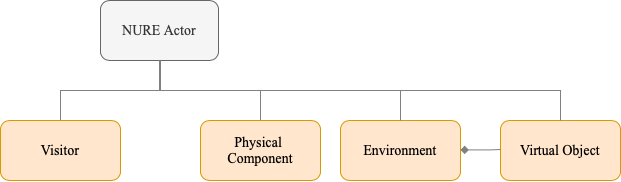
\includegraphics[width=14cm]{Figures/Conceptual Model/SM_NURE1.png}
	\caption{Actors - NURE}
	\label{fig:ActorsNURE}
\end{figure}

\begin{figure}[H]
	\centering
	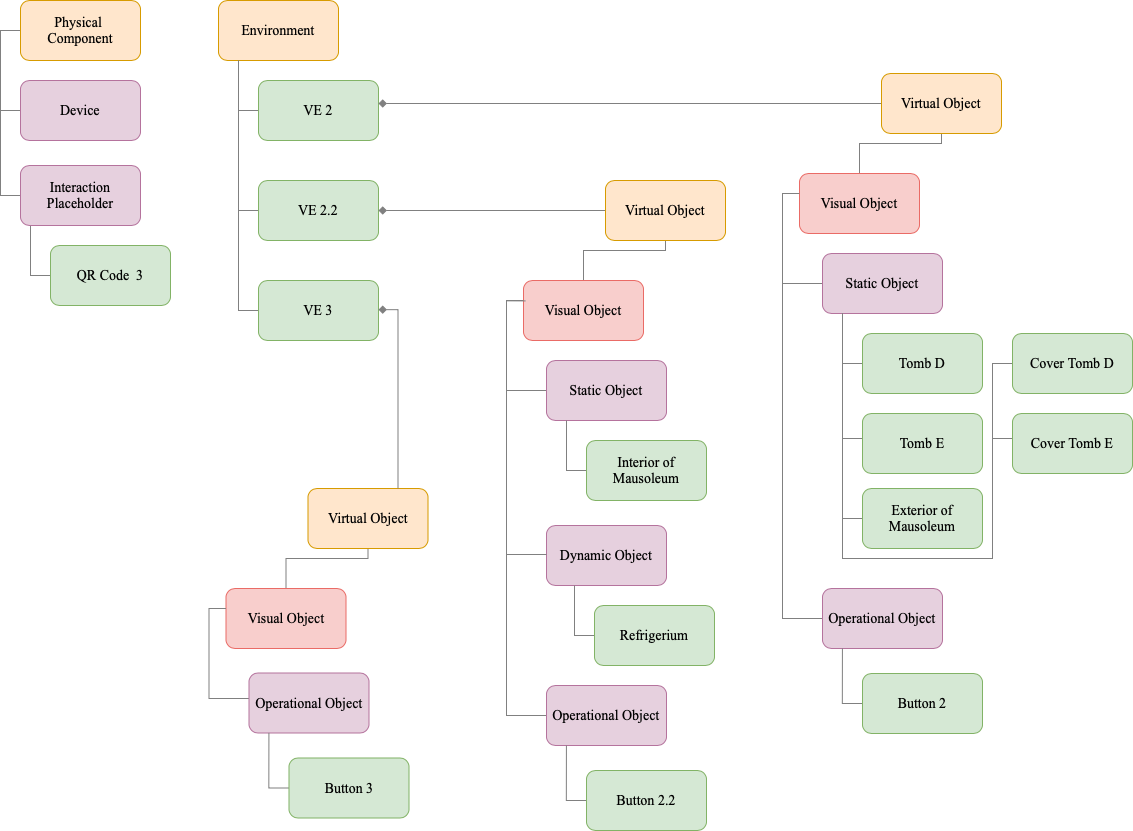
\includegraphics[width=14cm]{Figures/Conceptual Model/SM_NURE2.png}
	\caption{Non-Human Actors - NURE}
	\label{fig:NonHumanActorsNURE}
\end{figure}

\begin{itemize}
    \item \textbf{Physical Component}
    \begin{itemize}
        \item Device: it is not explicitly present in the reported case study, however it is included because the visitor experiences the whole site through a device such as a viewer, namely Hololens.
        \item QR Code: it has been classified as an Interaction Placeholder, being an element identifiable through the camera of a device. For each QR Code an ID is assigned. The Position property is not made explicit for reasons of simplicity. In NURE it is usually used to activate the Environment.
    \end{itemize}
    \begin{table}[h]
    \centering
    \begin{tabular}{|l|c|c|}
    \hline
    \textbf{Physical Component Properties} & \textbf{Device}     & \textbf{QR Code 3}    \\ \hline
    Position                               & \multicolumn{2}{c|}{\textit{not specified}} \\ \hline
    ID                                     & Hololens            & 3                     \\ \hline
    \end{tabular}
    \caption{Physical Component Properties - NURE}
    \label{tab:NUREPHCproperties}
    \end{table}
    \item \textbf{Environment}
    \begin{itemize}
        \item Augmented Environment: the experience is divided into several Augmented Environments. These represent scenes anchored in real world space augmented by the presence of Virtual Objects. The illustrated example starts from the visitor's entry into Augmented Environment 2 (AE 2) (Site zone 3. in \autoref{fig:ortophoto}), therefore after having already passed through Environment 1, which is indeed hidden. The Visitor continues through Environment 2.2 (AE 2.2)(Site zone 4. in \autoref{fig:ortophoto}) until entering Environment 3 (AE 3) (Site zone 5. in \autoref{fig:ortophoto}), thus after AE 2 has become hidden. 
        \autoref{tab:NUREAEproperties} does not go into detail with regard to the Position and Orientation properties of the Camera, even though both usually coincide with the observer's position.
    \end{itemize}
    \begin{table}[h]
    \centering
    \begin{tabular}{|l|l|l|l|}
    \hline
    \textbf{Environment Properties}           & \textbf{AE 2} & \textbf{AE 2.2} & \textbf{AE 3} \\ \hline
    Camera Position    & \multicolumn{3}{c|}{\textit{not specified}} \\ \hline
    Camera Orientation & \multicolumn{3}{c|}{\textit{not specified}} \\ \hline
    Visibility         & ON           & OFF           & OFF          \\ \hline
    \textbf{Augmented Environment Properties} & \textbf{AE 2} & \textbf{AE 2.2} & \textbf{AE 3} \\ \hline
    World Anchors      & \multicolumn{3}{c|}{\textit{not specified}} \\ \hline
    \end{tabular}
    \caption{Augmented Environment Properties - NURE}
    \label{tab:NUREAEproperties}
    \end{table}
    \item \textbf{Virtual Object}
    \begin{itemize}
        \item 3D Model: it belongs to the Static Objects and is a 3D holographic representation of some of the elements that were part of the archaeological site and that have been reconstructed using computer graphics to allow visitors to learn about some of the objects of the past. 
        
        The AE 2 contains the Tomb D, the Tomb E (\autoref{fig:tombs}), the respective Covering slabs considered as a separate object in order to allow the user to move them and finally the Exterior of the Mausoleum (\autoref{fig:mausoleum}). The interior of the Mausoleum instead is part of AE 2.2, which also in this case is distinguished from the exterior in order to allow the visitor to observe the Mausoleum from both the outside and the inside. It is a design choice to separate the components and usually serves either to make the experience more interactive or to simplify the design as in the case of the Mausoleum which is layered to show the inside rather than to encourage the visitor to "walk inside".
        
        The 3D Models are anchored to the Augmented Environment and have an absolute position, orientation and scale that are not defined for reasons of simplicity. The initial state has been set considering that AE 2 has already been triggered and all 3D Models inside are Visible. 
        
        \begin{table}[h]
        \centering
        \resizebox{\textwidth}{!}{%
        \begin{tabular}{|l|c|c|c|c|c|c|}
        \hline
        \multicolumn{1}{|c|}{\textbf{Virtual Object Properties}} &
          \textbf{Tomb D} &
          \textbf{Tomb E} &
          \textbf{\begin{tabular}[c]{@{}c@{}}Cover \\ Tomb D\end{tabular}} &
          \textbf{\begin{tabular}[c]{@{}c@{}}Cover \\ Tomb E\end{tabular}} &
          \textbf{\begin{tabular}[c]{@{}c@{}}Exterior of\\ Mausoleum\end{tabular}} &
          \textbf{\begin{tabular}[c]{@{}c@{}}Interior of\\ Mausoleum\end{tabular}} \\ \hline
        Position &
          \multicolumn{6}{c|}{\textit{not specified}} \\ \hline
        Orientation &
          \multicolumn{6}{c|}{\textit{not specified}} \\ \hline
        \multicolumn{1}{|c|}{\textbf{Visual Object Properties}} &
          \textbf{Tomb D} &
          \textbf{Tomb E} &
          \textbf{\begin{tabular}[c]{@{}c@{}}Cover \\ Tomb D\end{tabular}} &
          \textbf{\begin{tabular}[c]{@{}c@{}}Cover \\ Tomb E\end{tabular}} &
          \textbf{\begin{tabular}[c]{@{}c@{}}Exterior of \\ Mausoleum\end{tabular}} &
          \textbf{\begin{tabular}[c]{@{}c@{}}Interior of\\ Mausoleum\end{tabular}} \\ \hline
        Geometry &
          3D &
          3D &
          3D &
          3D &
          3D &
          3D \\ \hline
        Visibility &
          ON &
          ON &
          ON &
          ON &
          ON &
          OFF \\ \hline
        Scale Factor &
          \multicolumn{6}{c|}{\textit{not specified}} \\ \hline
        Opacity &
          100\% &
          100\% &
          100\% &
          100\% &
          50\% &
          0\% \\ \hline
        Selectable &
          ON &
          ON &
          ON &
          ON &
          ON &
          OFF \\ \hline
        Blinking &
          ON &
          ON &
          ON &
          ON &
          ON &
          OFF \\ \hline
        \multicolumn{1}{|c|}{\textbf{2D/3D Model Properties}} &
          \textbf{Tomb D} &
          \textbf{Tomb E} &
          \textbf{\begin{tabular}[c]{@{}c@{}}Cover \\ Tomb D\end{tabular}} &
          \textbf{\begin{tabular}[c]{@{}c@{}}Cover \\ Tomb E\end{tabular}} &
          \textbf{\begin{tabular}[c]{@{}c@{}}Exterior of \\ Mausoleum\end{tabular}} &
          \textbf{\begin{tabular}[c]{@{}c@{}}Interior of\\ Mausoleum\end{tabular}} \\ \hline
        Texture &
          Stone &
          Stone &
          Stone &
          Stone &
          Stone &
          Stone \\ \hline
        \end{tabular}%
        }
        \caption{3D Model Properties - NURE}
        \label{tab:NURE3DMproperties}
        \end{table}
        
        \begin{figure}[h]
        	\centering
        	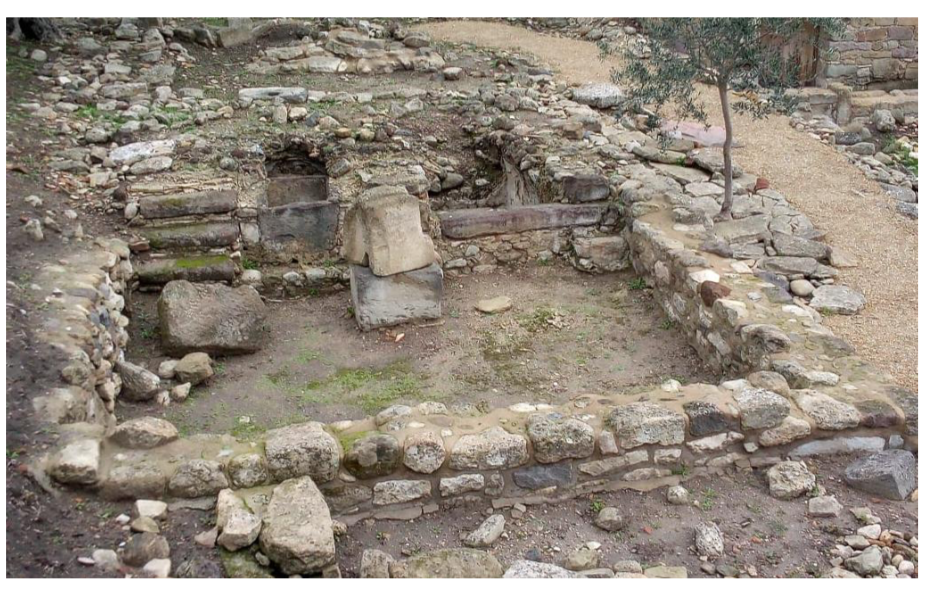
\includegraphics[width=\linewidth]{Figures/Conceptual Model/photoNURE/mausoleum.png}
        	\caption{Mausoleum - NURE}
        	\label{fig:mausoleum}
        \end{figure}
    
        \begin{figure}[h]
        	\centering
        	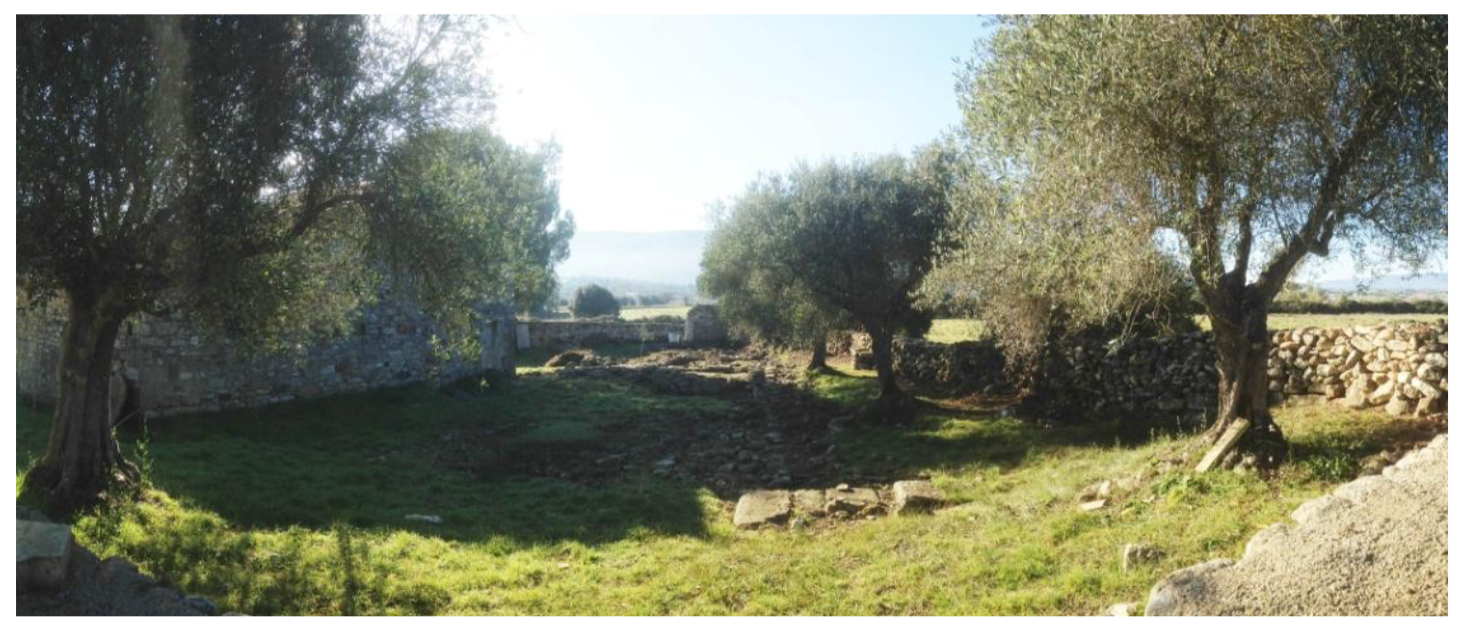
\includegraphics[width=\linewidth]{Figures/Conceptual Model/photoNURE/tombs.png}
        	\caption{Tomb D and Tomb E - NURE}
        	\label{fig:tombs}
        \end{figure}
        
        \item Video: it is included in the Dynamic Objects and is represented in NURE as an animated 3D model that reproduces scenes of everyday life from that historical period on a loop. 
        The visitor observes the reproduction of the Refrigerium ritual inside the Mausoleum: two women are standing in front of the tombs and two flames are lit. The first woman deposits the food content of the bowl in the first tomb and returns to her position. The second pours the liquid contents of the jug into the cup carved in the tomb in front of her. At the end the two women return to contemplate with their hands in prayer near their faces. Initially the 3D Video is not visible, it is activated later in AE 2.2.
        
        \begin{table}[h]
        \centering
        \begin{tabular}{|l|c|}
        \hline
        \textbf{Virtual Object Properties}                       & \textbf{Refrigerium}   \\ \hline
        Position                                                 & \textit{not specified} \\ \hline
        Orientation                                              & \textit{not specified} \\ \hline
        \textbf{Visual Object Properties}                        & \textbf{Refrigerium}   \\ \hline
        Geometry                                                 & 3D                     \\ \hline
        Visibility                                               & OFF                    \\ \hline
        Scale Factor                                             & \textit{not specified} \\ \hline
        Opacity                                                  & 0\%                    \\ \hline
        Selectable                                               & OFF                    \\ \hline
        Blinking                                                 & OFF                    \\ \hline
        \multicolumn{1}{|c|}{\textbf{Dynamic Object Properties}} & \textbf{Refrigerium}   \\ \hline
        Loop                                                     & ON                     \\ \hline
        Duration                                                 & \textit{not specified} \\ \hline
        \end{tabular}
        \caption{Video Properties - NURE}
        \label{tab:NUREVideoproperties}
        \end{table}
        
        \item Button: it is an Operational Object and is represented as a static 3D model that allows the visitor to choose which actions to perform among all those included in the 3D Menu. We have assigned each Button an ID which in this case coincides with the number that identifies each Augmented Environment. In NURE it is also used as an alternative to the QR Code to activate an Augmented Environment. 
        
        \begin{table}[h]
        \centering
        \begin{tabular}{|l|c|c|}
        \hline
        \textbf{Virtual Object Properties} & \textbf{Button 2}   & \textbf{Button 2.2}   \\ \hline
        Position                           & \multicolumn{2}{c|}{\textit{not specified}} \\ \hline
        Orientation                        & \multicolumn{2}{c|}{\textit{not specified}} \\ \hline
        \textbf{Visual Object Properties}  & \textbf{Button 2}   & \textbf{Button 2.2}   \\ \hline
        Geometry                           & 3D                  & 3D                    \\ \hline
        Visibility                         & ON                  & OFF                   \\ \hline
        Scale Factor                       & \multicolumn{2}{c|}{\textit{not specified}} \\ \hline
        Opacity                            & 100\%               & 0\%                   \\ \hline
        Selectable                         & ON                  & OFF                   \\ \hline
        Blinking                           & ON                  & OFF                   \\ \hline
        \end{tabular}
        \caption{Button Properties - NURE}
        \label{tab:NUREButtonproperties}
        \end{table}
    \end{itemize}
\end{itemize}

\subsubsection*{Behavioural Model - NURE}

\emph{User Actions and Effects}. The User Actions chosen for the visitors of the archaeological park, as well as participants in the NURE experience, and the Effects generated on the respective Non-Human Actors are illustrated in the following \autoref{tab:UAENURE}.
\begin{table}[h]
\centering
\begin{tabular}{|l|l|}
\hline
\textbf{User Aciton}    & \textbf{Effect}    \\ \hline
Tap                     & Visible            \\ \hline
Swipe                   & Hidden             \\ \hline
Proximity Out           & Hidden             \\ \hline
\multicolumn{1}{|c|}{-} & Visible \& On Play \\ \hline
Tap                     & Hidden             \\ \hline
Object Recognition      & Visible            \\ \hline
Object Recognition      & Hidden             \\ \hline
\end{tabular}
\caption{User Action \& Effect combination - NURE}
\label{tab:UAENURE}
\end{table}

The designed Effects can be achieved by performing different alternatives of User Actions. The choice is up to the experience designer who takes into account the device in use. Gestures are a form of input on HoloLens. Once you point at a hologram with your gaze, the visitor can interact with that hologram with a gesture. A user targets an item with their gaze and then selects or activates the target with a gesture. When a user places their hand in the field of view they get an activation event indicating that the user is ready for input.
In Hololens, what we have called Tap corresponds to mouse click and can be used to take an action on the currently targeted item. When the device sees the user's hand, a floating pointer appears near the tip of the index finger to help point at items. 

The gestures used in NURE are a natural and intuitive way for Visitors to interact with mixed reality content. For example the Tap on a Button can make Visible or Hidden an Environment, the Proximity Out to the Environment can hide the Virtual Objects contained in it. Another important User Action identified in this model is Object Recognition and corresponds to the "frame" gesture in HoloLens 2. It has sensors that can see a few meters on each side of the user. To identify objects like the QR Code, you have to hold them within that frame and as the user moves, the frame moves with them. 

The Effects created for the NURE case study are shown in \autoref{fig:IM1NURE} and \autoref{fig:IM2NURE}. It has been decided to show them in the next section in order to include them in the building blocks that constitute the Tasks, represented respectively by the Interaction and the System Event. 
The only Effect that does not have a corresponding User Action is the Visible \& On Play combination, generated via a System Event that will be modelled in the next section. 

\subsubsection*{Interaction Model - NURE}

\emph{Interaction and System Event}. \autoref{fig:IM1NURE} and \autoref{fig:IM2NURE} show how the Interaction and System Event blocks have been constructed, sided by the related Effect blocks visible on the Actuators. 

\begin{figure}[h]
	\centering
	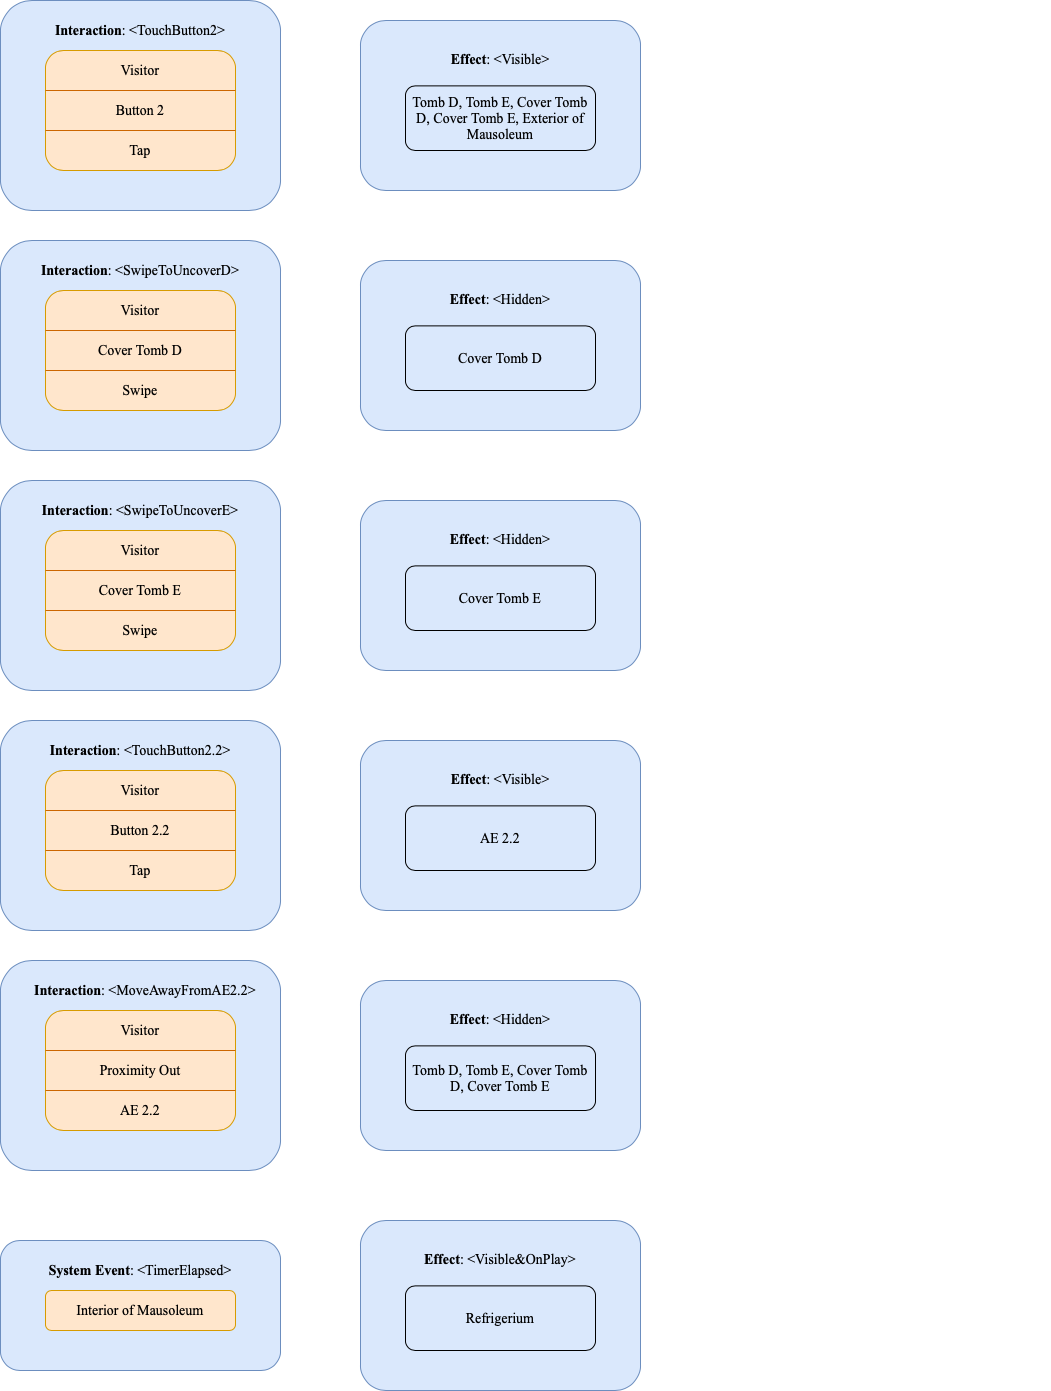
\includegraphics[width=14cm]{Figures/Conceptual Model/IM_NURE.png}
	\caption{Interaction, System Event \& Effect combination - NURE}
	\label{fig:IM1NURE}
\end{figure}
\begin{figure}[h]
	\centering
	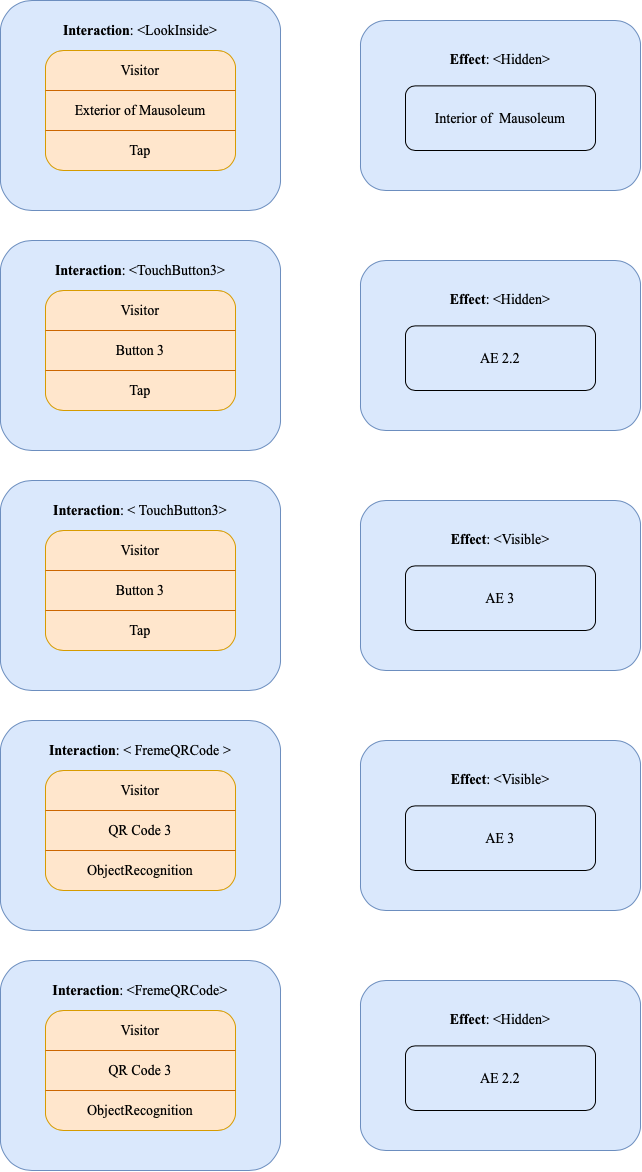
\includegraphics[width=12cm]{Figures/Conceptual Model/IM_NURE2.png}
	\caption{Interaction, System Event \& Effect combination - NURE}
	\label{fig:IM2NURE}
\end{figure}

Each Interaction block is associated with an Effect: the block includes the Human Actor (top box of the block), who performs the action(s), the User Actions (middle box of the block) and the Target(s) (bottom box of the block). For example, the visitor can tap on Button 2 and make the Virtual Objects (Actuators) visible, such as Tomb D, Tomb E, the respective Cover E and Cover D and the Exterior of Mausoleum. Subsequently, the visitor moving away from AE 2 causes the Virtual Objects (Actuators) to become Hidden from Visible. The properties owned by the Actuators change when they undergo an effect. 
From \autoref{tab:NURE3DMproperties} it can be seen that initially Tomb D, Tomb E, their respective Cover E and Cover D and the Exterior of Mausoleum had the \textit{Visibility}, \textit{Selectable}, \textit{Blinking} properties set to ON and \textit{Opacity} set to 100\%. The Hidden Effect has changed these properties to \textit{Visibility}, \textit{Selectable}, \textit{Blinking} set to OFF and \textit{Opacity} set to 0\%. 
The same reasoning applies to all combinations of Interactions/System Events with their corresponding Effects.

The System Event block is also associated with an Effect: the block only includes the Target(s) in one box. The example shows how the "time expired" event set on the Interior of Mausoleum generates the playback of the Refrigerium video.

\emph{Task and Activity}. At this stage, having defined all the necessary components, we move on to the configuration of the Tasks and Activity. The Tasks include both several Interactions involving the visitor exploring the Environment and its Virtual Objects and also a System Event determined by the expiration of a Timer. \autoref{fig:ActivityNURE} shows the Activity as a flowchart in which the Tasks are represented in a compacted way, therefore less detailed for obvious reasons of space. To explain the Activity in detail we use a procedure like a Use Case Scenario. 
\begin{figure}[h]
	\centering
	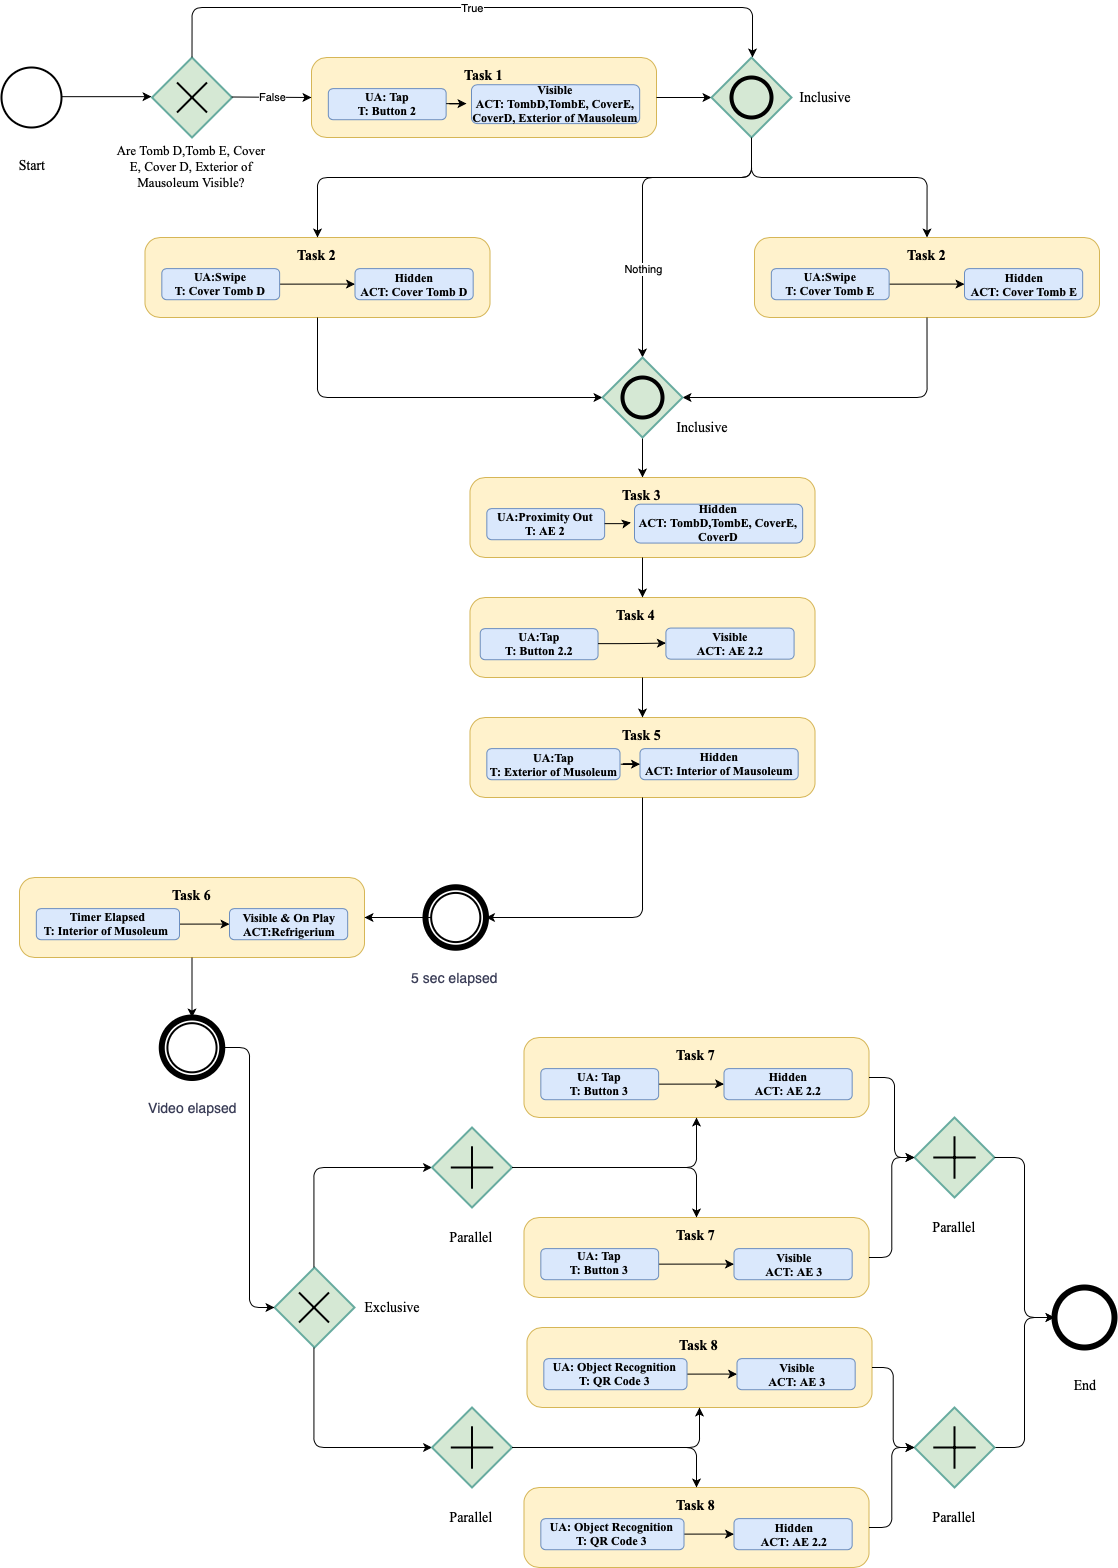
\includegraphics[width=16.5cm]{Figures/Conceptual Model/NUREExample.png}
	\caption{Activity Flow - NURE}
	\label{fig:ActivityNURE}
\end{figure}
Stefano is a 24-year-old guy studying Computer Engineering in Milan who loves art and technology. He has recently heard about the opening of the NURE Archaeological Park in its 2.0 edition. Stefano doesn't want to miss the opportunity to visit an ancient historical site that he studied in books as a child and that now seems to have taken on a completely new form thanks to the introduction of MR. He has used viewers before, but this is the first time he is using Hololens 2, which makes him very excited. 

Once in Sardinia, Stefano goes to the nuragic complex and waits his turn to visit. 
The tour starts inside the Paleochristian church which coincides with the first Augmented Environment (AE 1) containing a nuraghe and a hut. 
Stefano, at this point, is already quite confident with the Hololens technology and approaches the AE 2 which is activated together with all its three-dimensional elements. It is the second Activity and Stefano fortunately does not need to activate, manually through the Tap of Button 2, the single Virtual Objects (the Tomb D, the Tomb E, the respective Cover E and Cover D and the Exterior of Mausoleum). Stefano sees them all blinking at different distances from him and since Tomb D and Tomb E are the closest he has four options to choose from: 
\begin{enumerate}
    \item Explore Tomb D, by Swiping on the cover plate it will become transparent (i.e. Hidden), allowing him to look inside Tomb D.
    \item Explore Tomb E, by Swiping the cover plate it will become transparent (i.e. Hidden), allowing him to look inside Tomb E.
    \item Explore both Tombs, so first point 1. (or point 2.) and then choose point 2. (or point 1.) 
    \item Continue straight ahead (route "Nothing" in the Figure) without exploring either Tomb. 
\end{enumerate}
Stefano chooses option 2. and proceeds to move away from AE 2. The Hololens he is wearing has detected the distance from AE 2 so the Virtual Objects contained therein will become Hidden except for the Exterior of Mausoleum. Using Button 2.2 he activates the new Environment 2.2. 
Finally Stefano can explore the Mausoleum inside, by tapping on the Exterior of Mausoleum which becomes transparent. 
With great surprise after only 5 seconds (Intermediate Event) a scene of an ancient rite is played: the Refrigerium. The video ends and Stefano is really moved for having relived a glimpse of the past. 
To activate the AE 3 Stefano is again faced with a choice: between framing with the Hololens the QR code 3 and tapping on the button 3 of the Menu he chooses the first option. The AE 3 becomes Visible for Stefano while the AE 2.2 is Hidden together with all its components. 
